\documentclass[a4paper, 12pt]{article}

% Paragraph settings
\setlength{\parskip}{1em}
\setlength{\parindent}{0em}

% Allow subfiles for sections
\usepackage{subfiles}

% Allow hyperlinks
\usepackage{hyperref}

% Allow URLs in references
\usepackage{url}

% Allow using \linewidth
\usepackage{graphicx}
\graphicspath{{images}{../images/}}

% Allow float position for figures
\usepackage{float}

% Allow inclusions of files verbatim
\usepackage{verbatim}

% Figures with bold labels
\usepackage[labelfont=bf]{caption}

% Allow colored text
\usepackage[usenames,dvipsnames,svgnames,table]{xcolor}

\begin{document}

\begin{center}
    {\huge Reflective Journal \par}
    {\large Ashley Stewart\par}
    SEB403 - Honours Research Project
\end{center}

\tableofcontents

\newpage
{\large\textbf{Legend}}

\textbf{Black:} What happened 

\textcolor{Blue}{\textbf{Blue:} Reflections}

\textcolor{Magenta}{\textbf{Magenta:} Future planning and decisions}

\vspace{8mm}

{\large\textbf{Decision-making process}}
\begin{enumerate}
  \item{Identify the decision}
  \item{Gather information}
  \item{Identify options}
  \item{Weigh the options}
  \item{Choose an option}
  \item{Take action}
  \item{Evaluate and review}
\end{enumerate}

\newpage
\section{Log: VRES (January-February)}
From early January to late February, I participated in QUT's \emph{Vacation Research Experience Scheme} (VRES), where I met Dr Donald Dansereau, who would later supervise me throughout my Honours studies. The project I was a part of was called \emph{Robotically Assisted Surgery}.

When I began, Donald introduced the notion of a Light Field to me, \textcolor{Blue}{which I found fascinating, especially after he linked it with the surgical application. The area was not familiar to me,} but Donald set out a range of written material for me to read to learn more. \textcolor{Blue}{I had never read a research paper in full before, so this was a new skill for me that took time to develop. }\textcolor{Magenta}{It was very useful to have some of these skills before my Honours studies began, especially for my semester one Literature Review.}

Alongside the readings, I was handed the Raspberry Pi camera array to familiarise myself with. The camera array was built using Raspberry Pi devices networked together. \textcolor{Blue}{Luckily, I had some experience working with Linux and Raspberry Pis in my undergraduate years.} Interfacing and experimenting with them took time at first (we didn't actually know how to connect to them via the network), so once I had everything up and running, \textcolor{Magenta}{I decided to take the liberty of writing up some brief documentation describing my methods.} \textcolor{Blue}{This documentation may be useful to any future students who use the device.}

Once I was familiar enough with the Raspberry Pi devices, and had read most of the literature Donald compiled for me, \textcolor{Magenta}{we had a discussion about research direction. There were several areas that I could have gone into, but the one that seemed most interesting to me was the idea of occlusion removal techniques for light field cameras, possibly involving light field video.}

\textcolor{Blue}{In retrospect, I very much wish I attempted some of the methods described in the research papers Donald put together for me during VRES. Even if every attempt was incorrect, I would have learned a lot from experimentation, and from Donald's feedback. I likely would have made significant progress at an earlier stage in Honours.} Instead, most of my time was spent attempting to generate synchronised live video streams, testing out potentially useful software on the Raspberry Pis, and other pursuits.

Towards the end of VRES, I was required to present my VRES experience as an oral presentation to the other VRES students in the faculty. \textcolor{Magenta}{After some discussion with Donald, we decided this was a good opportunity to develop a research proposal for my Honours studies.} \textcolor{Blue}{This was an excellent way to encourage me to practice writing, sourcing literature, and otherwise compile materials together to form a coherent intention with the presentation.} The written proposal that accompanied the presentation was a short proposal, which outlined the motivation and aims. \textcolor{Blue}{The methodology descriptions were very minimal at that stage, because I was still learning a lot about the topic, and was not at the stage where I could confidently state a process.}

\textcolor{Blue}{My VRES experience was an excellent introduction to the research area and the resources I would later need. I wish that I had taken more advantage of the opportunity by attempting to prepare a concrete implementation.}

\newpage
\section{Log: March}
This month, I officially began my Honours studies after my entry proposal was accepted.

By attending lectures and classes, \textcolor{Blue}{I developed a greater understanding of how to structure technical written material, especially a literature review.} \textcolor{Magenta}{This of course would be very useful for my future assessment items.}

To prepare for these assessment tasks, I also continued compiling papers for the literature review. Mostly, they were papers suggested by Donald. I spent lots of time reading these papers, writing notes about them and summarising them, \textcolor{Magenta}{so that I could develop some way to organise them into the literature review.}

\textcolor{Blue}{Although I understood the papers from a surface level, and could draw out the clear overall differences between their intention, I still was not confident implementing the procedures they described. I was not used to the heavy theoretical descriptions, and struggled with taking the first step to apply them in an implementation.} Therefore, I did not achieve any significant project work this month.

Finally, I spent some time working with the Raspberry Pi camera array, attempting to capture synchronised images \textcolor{Magenta}{which would be necessary as the project developed further in future.}

Outside of my research work, I was working two jobs - one as an academic tutor, and one as an website administrator. \textcolor{Blue}{It is clear looking back that this affected my work output, and continued to until mid-May,} when I decided to resign from the website administrator position.

\newpage
\section{Log: April}
This month, I learned more about writing a formal project proposal. \textcolor{Blue}{The original proposal I wrote for Honours entry would not do for assessment, as it was very brief and vague.}

This month I was very focused on the literature review, and had a lot of back and forth with Donald about papers. \textcolor{Blue}{This was a very productive time for me in terms of my understanding of concepts, because I found many relevant research papers on my own, and discussed their ideas with Donald.}

In relation to my work with the Raspberry Pi camera array, some significant problems presented themself. \textcolor{Magenta}{Donald, myself and Steven organised to meet on several occasions to discuss the problems and decide on possible solutions. We eventually had good ideas for the way forward, and I made a point of suggesting concrete dates to achieve things by.} Specifically, we were organising the production of a new aluminium front-plate for the camera array, to ensure a stable camera setup.

\newpage
\section{Log: May}
\textcolor{Magenta}{Because I was waiting on the production of the new front-plate, I decided to put off doing any real project work this month in favour of completing my literature review. I also had to complete a large assignment for another coursework unit (AI for Games).}

Donald provided the following feedback about the literature review: 

\textcolor{Blue}{\emph{"Ashley has undertaken a complex project in an area unfamiliar to him. In formulating his literature review and proposal he has effectively taken in a wide range of new material, spanning camera calibration, video filtering, occlusion removal, and light field processing. Starting from a handful of paper recommendations, he has taken a proactive approach to finding new, relevant works and incorporating their content into the project plan. He has made excellent progress in this regard.}}

\textcolor{Blue}{\emph{Progress in actually building the elements of the project has been slow. It seems this is partly a function of the way the class is structured, with the proposal only due very recently. Given the complexity of the work, I would have liked to see more emphasis on progressing the technical elements early on. With the literature review and proposal complete, I expect that technical progress can begin in earnest.}}

\textcolor{Blue}{\emph{Despite the slow early technical progress, his success in tackling complex subject matter makes me confident that Ashley will be able to develop his ideas into an impressive demonstration and deliver on the key goals of the project."}}

\textcolor{Blue}{I wholly agreed with Donald's points, especially the final ones about achieving technical progress, but I felt encumbered by the wait to build the replacement front-plate for the camera array.} \textcolor{Magenta}{I thought it would be best to ensure this semester I spend time ensuring a solid literature review and project proposal, with the majority of project work taking place in semester two.} \textcolor{Blue}{In retrospect, I believe if I had the courage to attempt some technical work, I may have made significant progress, the results of which would only show more when the front-plate was replaced. Achieving such work early on may have even improved the quality of my project proposal, as it would likely assist me in describing the process and implementation.}

\section{Log: June}
This month, which was the final month of semester one, my main focus was on completing the project proposal. \textcolor{Blue}{I found it relatively easy to discuss the applications, relevant literature, and research gap, but continued to have some difficulty with describing the complete methodology, since the research topic is largely exploratative.} After some discussions with Donald, I put together a concrete methodology for camera calibration and rectification, but only various options for possibilities with occlusion removal. \textcolor{Blue}{Again, I feel this was, at least in part, due to a lack of experience completing such technical work in practice. It was relatively easy to decide on a calibration procedure after discussions with Donald, because the camera array largely dictates which methods will work best. The occlusion removal area on the other hand, which was also the main research area discussed in the proposal, was very experimental, and so in the proposal I listed options for where the project may go in semester two.}

\textcolor{Magenta}{As part of my project proposal, I developed a basic timeline for semester two to act as a model for project work (see figure~\ref{fig:timeline}). It was important to lay out such a timeline to ensure that project work is achieved, given the now limited timeframe.} Note how the front-plate is replaced early on, along with camera calibration taking place shortly after. Later on the timeline are various demonstration dates, which are discussed in more detail in the proposal.

\begin{figure}[H]
    \centering
    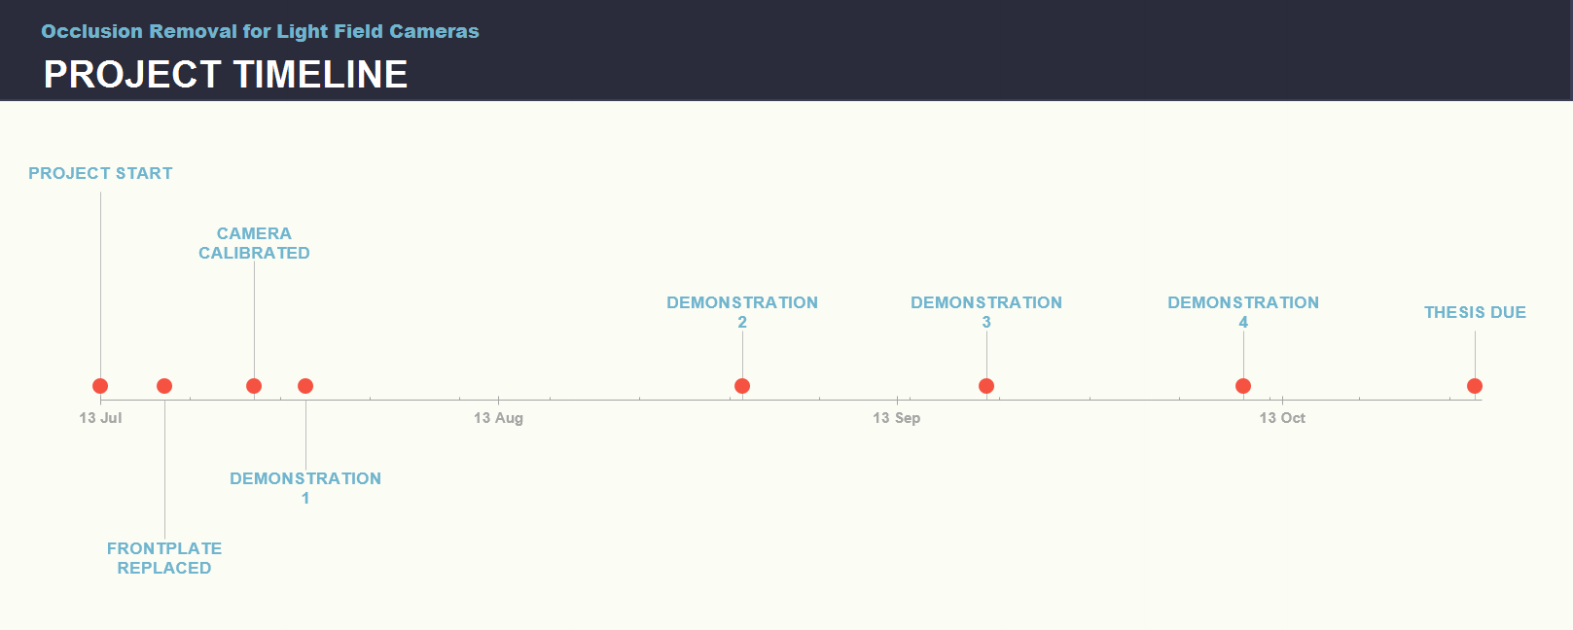
\includegraphics[width=\linewidth]{images/timeline}
    \caption{Semester two project timeline as it appears in the Project Proposal.}
    \label{fig:timeline}
\end{figure}

\section{Log: August}
This month, I finally achieved some significant project work. After a few weeks of resoldering and adjusting the camera array's power setup, I eventually had all the camera modules working on the 19th of August. \textcolor{Blue}{At this point, I was worried about whether I would be able to achieve an outcome for the project in time,} \textcolor{Magenta}{and suggested to Donald that I may need to change my goals from the original proposal.} Donald's reponse was as follows:

\emph{\textcolor{Blue}{"Nice work getting everything up and running. I appreciate that you have tackled some new challenges, and am glad to see you take on some new skills.}}

\emph{\textcolor{Magenta}{In terms of a plan, what you suggest sounds reasonable.  I would suggest getting a minimal focus example working using checkerboards to calibrate. Perhaps follow a simplified procedure, e.g. plane + parallax. Then decide if you want to spend time making it fast on the RPis, or extend the functionality, e.g. by adding tracking through depth, or experimental results involving occlusions."}}

After considering Vaish's plane + parallax procedure which Donald suggested, I discovered that it does not take into account rotation between cameras, which I could tell would be significant. Donald then suggested:

\emph{"Consider checking out my PhD Dissertation Section 6.3, up to and including 6.3.2. The methods are not that different, I just wrote in more detail. Also, you can carry out effectively the same thing by extending the panoramic stitching code from the matlab examples."}

I eventually found that Donald's method, though it wasn't a formal calibration procedure, could be extended to provide a conceptually simple calibration, that was also flexible to camera rotation. If formalised, tested and evaluated, this would prove to be a novel outcome. So, I finally began developing and testing concrete implementations of a procedure by referring to Donald's PhD and panoramic stitching code. \textcolor{Blue}{The results here were mixed, but represented significant progress in my confidence and abilities, since I was actively developing and testing.} \textcolor{Magenta}{If I continued with the same vigor, I would surely achieve some good quality results in the near future.}

\section{Log: September}
This month, I achieved significant demonstrations in light field rendering using the Raspberry Pi camera array, including synthetic aperture focusing on the 20th of September. Robustness to occlusion was also demonstrated. \textcolor{Blue}{This was a result of continuous development and testing.}

\textcolor{Blue}{Although good results were achieved here,} \textcolor{Magenta}{for my thesis, I still needed to think about how to formalise the calibration into a process, and think about the factors that enabled the results.}

\textcolor{Magenta}{As for any further project work, I was unsure of where to go from here, so I discussed this with Donald. His response was as follows:}

\textcolor{Magenta}{\emph{"Moving forward: I'd suggest exploring the ideas in the proposal and things we've discussed. A video demo of seeing around occluders; a better way to see around occluders; joint space/time filtering. Many options, I hope you'll have time to explore one of these topics with in depth."}}

\textcolor{Magenta}{Unfortunately as we were very close to the due date, I did not want to risk implementing anything that required additional conceptually complex implementations. My efforts would be better spent refining my existing calibration procedure. However, one of Donald's suggestions - light field video, could be demonstrated along with the same synthetic aperture focusing approach used to see through occluders in light field stills.}

I spent the rest of my time this month working on refining the existing calibration and rectification implementations, and working towards light field video, which I achieved a rough demonstration of on the 30th of September. \textcolor{Blue}{It was a success!} \textcolor{Magenta}{Now I will need to write up my thesis, measure results and evaluate.}

\newpage
\section{Log: October}
I spent the first part of this month focusing on my advanced unit project, which is unrelated to this research project.

From mid-October, I spent more time capturing light fields to form demonstrations for the thesis and presentation, and to calculate quantitative results from. Towards the end of this month, I actually began writing the thesis, and attempted to formalise the procedure into theory.

\textcolor{Blue}{Few decisions were made around this time, because most of my work continued steadily and 'according to plan'.} 

\section{Log: November}
From the very start of this month, and up until the due date, I regularly sent my thesis work to Donald for suggestions. \textcolor{Blue}{In these last few weeks, my writing and structure of my thesis improved dramatically after following Donald's suggestions.} 

On Friday the 4th, I had to present my main findings as an oral presentation. \textcolor{Blue}{Preparing this presentation was a fantastic way for me to bring everything together with a coherent intention that can be understood by others.} \textcolor{Magenta}{It was also an excellent way to refine my thesis in the final days before the due date.}

Shortly after the presentation, I discovered that the performance of my calibration procedure could be significantly improved by running multiple passes. \textcolor{Magenta}{I decided that it was absolutely worthwhile to recreate some of the earlier demonstrations using the multi-pass procedure, and describe the procedure in my paper.} \textcolor{Blue}{Luckily, I was able to complete this in time and was very happy with the final outcome and integration into the paper.}

\newpage
\section{Final reflections}
\textcolor{Blue}{I am very happy with the final project work completed during my Honours year. I feel that I have come a long way since the beginning, and I am now significantly more confident in my research skills, as well as technical comprehension and application.}

\textcolor{Blue}{I feel that if I were to start a project of similar technical complexity, I would have much less trouble, since I now know and better understand the research process, and have reflected on my work from this year. A major problem for me early on, was that I did not have the confidence to attempt concrete implementations for some time - I always felt as though I needed to \emph{learn more} or \emph{understand more}, and I used excuses to procrastinate achieving results. I realise now that any work is better than no work, and that a failed attempt does not represent a failure. My skills improve with practice, and I look forward to continuing to grow this way in future.}

\textcolor{Blue}{I am thankful to have had such a knowledgeable and helpful supervisor, and I very much look forward to continuing research in the near future.}

\end{document}